\documentclass{beamer}
\setbeamertemplate{navigation symbols}{}

\usepackage{beamerthemeshadow}
\usepackage{amsmath}
\usepackage{bm}

\begin{document}
\title{Information bounds and attractor dynamics of a Hebbian associative memory}  
\author{Clayton Seitz}
\date{\today} 

\begin{frame}[plain]
\titlepage
\end{frame}

\section{Introduction} 

\begin{frame}[plain]
\frametitle{Introduction} 

\end{frame}

\begin{frame}[plain]
\frametitle{RNNs trained with Hebbian learning rules}

\begin{center}
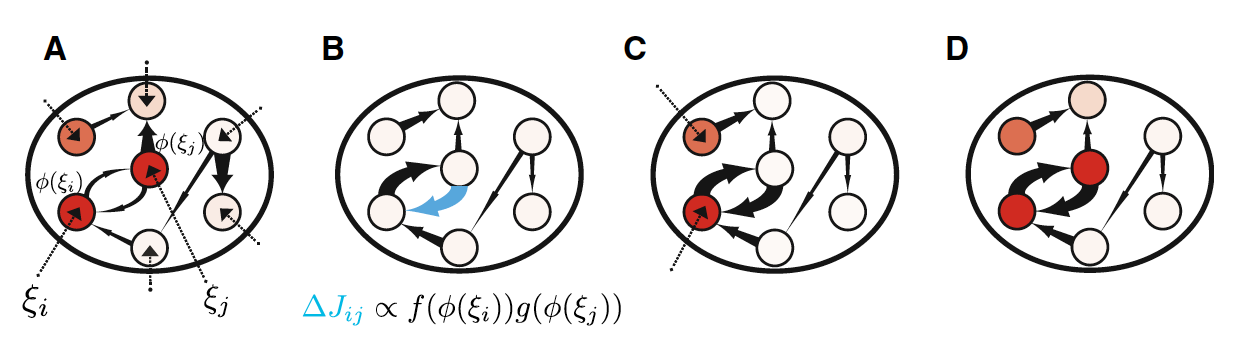
\includegraphics[scale=0.5]{network-diagram}
\end{center}

Let $W_{ij}$ be a matrix of recurrent weights that evolves when stimulated by 

\begin{equation*}
\xi(\bm{\mu}, \bm{\Sigma}) = \frac{1}{(2\pi)^{n/2}|\bm{\Sigma}|^{1/2}}\exp-\frac{1}{2}(\bm{r}-\bm{\mu})^{T}\bm{\Sigma}^{-1}(\bm{r}-\bm{\mu})
\end{equation*}

\footnote{\cite{peirera}}

\end{frame}
\begin{frame}[plain]
\frametitle{Inferring learning rules from firing rate distributions in ITC}

\begin{center}
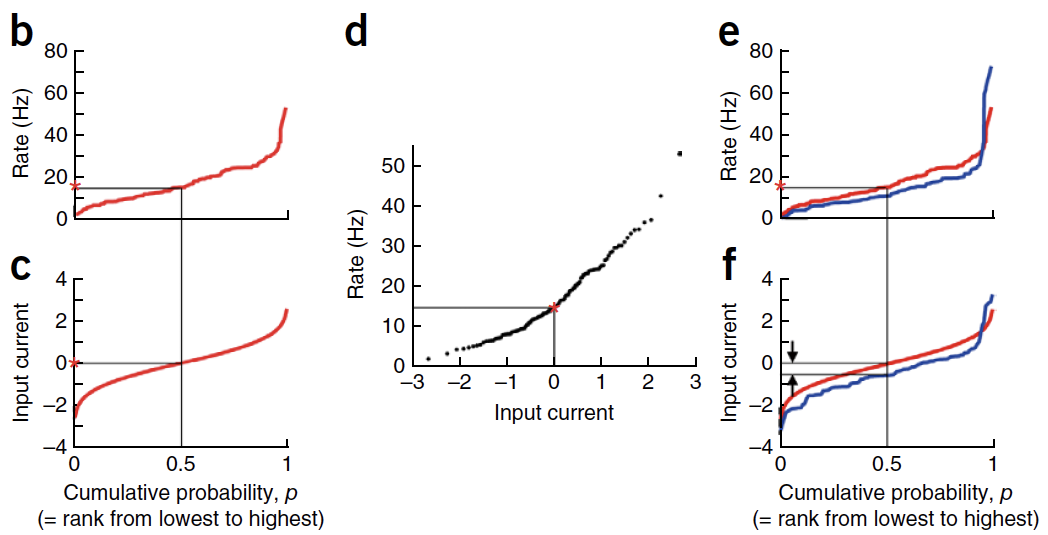
\includegraphics[scale=0.5]{learning-rules}
\end{center}

Inferring $\Delta W_{ij}$ from ITC neurons after presentation of novel and familiar images
\footnote{\cite{lim}}

\end{frame}

\begin{frame}[plain]
\frametitle{Inferring the transfer function from ITC data}

\vspace{0.2in}
All you can really observe is the firing rate distribution. Assume the input currents are Gaussian 

\begin{center}
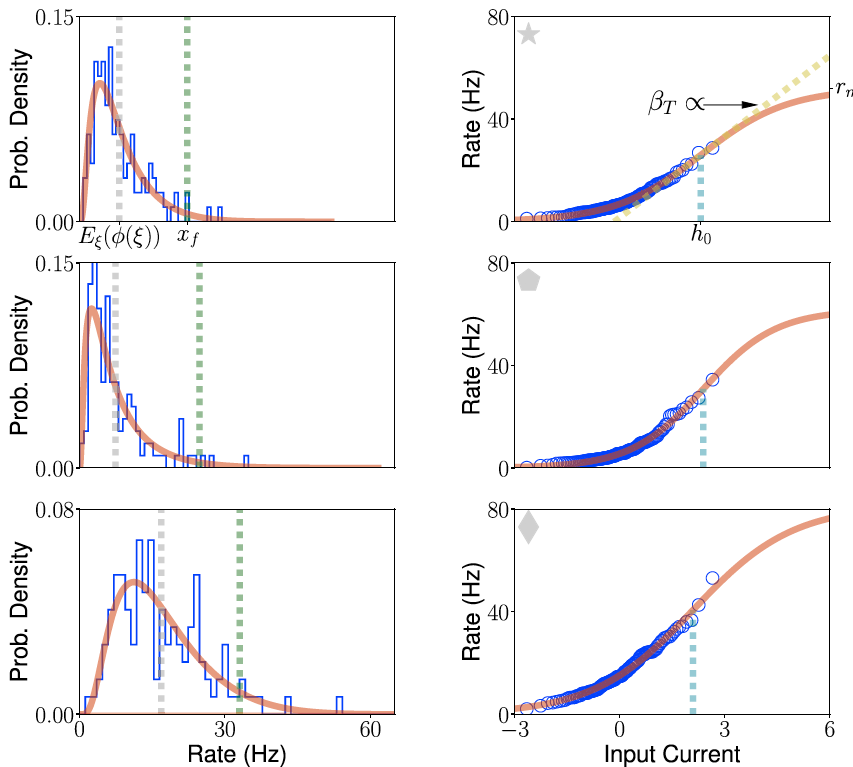
\includegraphics[scale=0.45]{transfer-function}
\end{center}

\footnote{\cite{peirera}}
\end{frame}

\begin{frame}[plain]
\frametitle{Presenting novel and familiar stimuli to the network}

\vspace{0.2in}

\begin{center}
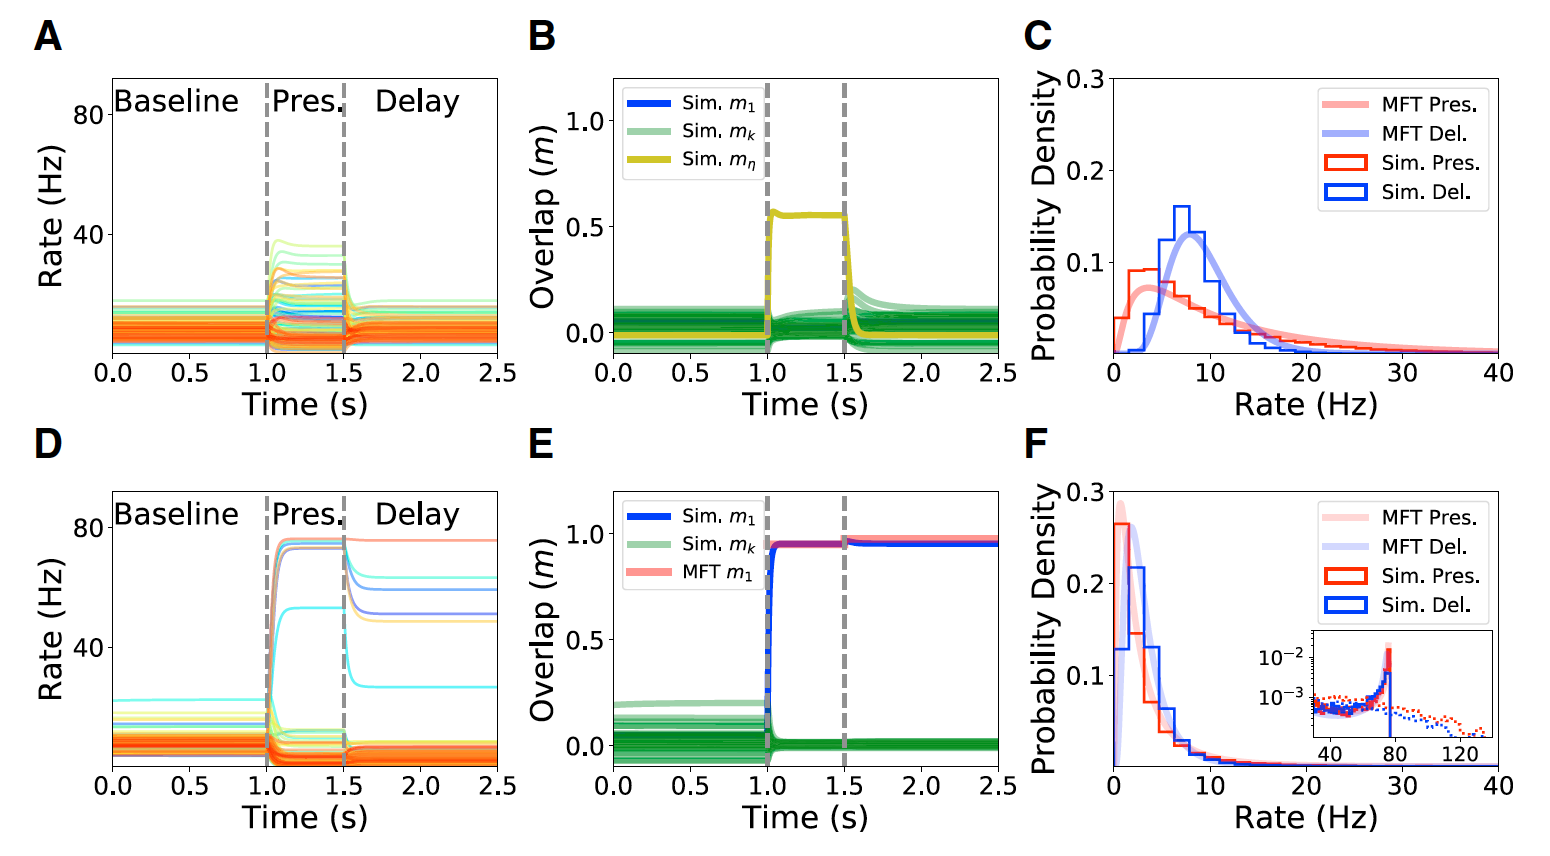
\includegraphics[scale=0.4]{novel-familiar}
\end{center}

\footnote{\cite{peirera}}

\end{frame}

\begin{frame}[plain]
\frametitle{A Hebbian update for synaptic weights}

Let the synaptic update be a separable function of the presynaptic $(\xi_{i})$ and postsynaptic $(\xi_{j})$ firing rates

\begin{equation*}
\Delta W_{ij} = f(\phi(\xi_{i}))g(\phi(\xi_{j})) \rightarrow W_{ij} = C_{ij}\sum  f(\phi(\xi_{i}))g(\phi(\xi_{j}))
\end{equation*}

\vspace{0.2in}

Evolution of the firing rate for neuron $i$ is

\begin{equation*}
\tau \dot{r_{i}} = -r_{i} + \phi(I + \sum_{j\neq i} W_{ij}r_{j})
\end{equation*}


\footnote{\cite{hopfield}}
\end{frame}


\begin{frame}[plain]
\frametitle{Do these networks optimize information transmission?} 

Are these networks functioning at a critical point? What about the balance between input and recurrence? (Cramer et al. 2020)

\begin{center}
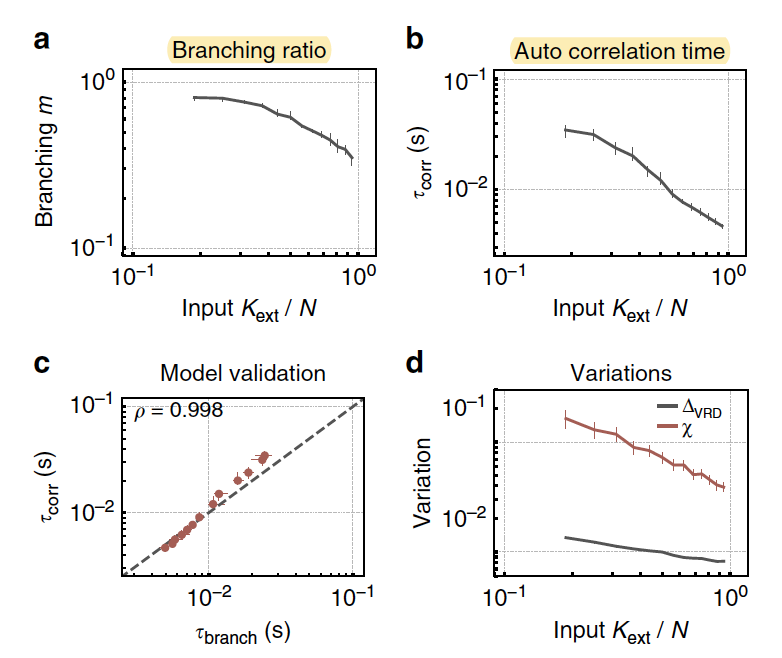
\includegraphics[scale=0.55]{cramer-criticality}
\end{center}

\end{frame}


\begin{frame}[plain]
\frametitle{A coding theory perspective} 

How much information does the response $R$ carry about the input pattern $S$ i.e. $I(R;S)$ on novel and familiar stimuli?

\vspace{0.2in}

What is the fundamental coding capacity of these networks?

\end{frame}


\begin{thebibliography}{99} 
\bibitem[Peirera and Brunel, Neuron. 2018]{peirera}
\bibitem[Lim et al., Nature Neuroscience. 2015]{lim}
\bibitem[J.J. Hopfield PNAS. 1982]{hopfield}
\end{thebibliography}






\end{document}